\section{Fourier Series}

With our newfound toolbox, we will investigate solving types of differential equations with an underlying periodic structure.  Specifically, we will consider now linear differential equations on the region $\Omega = [0,L]$ with periodic boundary conditions.  That is, we will be given some differential operator $\linop$, a function $g$, and we will be asked to solve for an $f$ such that
\begin{equation}
\label{eq:operator_diffeq}
\linop f = g,
\end{equation}
with $f$ subject to the boundary conditions $f(0)=f(L)$.  We refer to these boundary conditions as \boldgreen{periodic boundary conditions}.  Another way to view this problem is as defining the function $f$ to be continuous on a circle domain.  This point of view shows its head in the solution for the hydrogen atom.

For the sake of example, we will take the operator $\linop = -\frac{d^2}{dx^2}$ which is referred to as the 1-dimensional \boldgreen{Laplace operator} or \boldgreen{Laplacian}.  To follow the methodology outlined in the previous chapter, before we approach \ref{eq:operator_diffeq}, we must find the spectrum of $\linop$.  Hence, we must solve the eigenvalue equation
\[
\linop f = \omega^2 f,
\]
where $\omega^2$ is some constant that was chosen to simplify the later notation.  Thus, we arrive at the differential equation
\begin{equation}
\label{eq:harmonic_osc_operator}
-\frac{d^2}{dx^2}f(x) = \omega^2 f(x) \qquad\textrm{with~} f(0)=f(L).
\end{equation}
We have in fact solved this equation before! This is the harmonic oscillator equation with angular frequency $\omega$.  However, there is a difference.  In the previous case, we had a distinct and predetermined value for $\omega$ that was given by the system we were investigating (e.g., the stiffness of a spring).  Now, we allow $\omega$ to be a parameter for the problem as well.  

When we solved the matrix eigenvalue problem
\[
[A]\evec = \lambda \evec
\]
we wanted to take the determinant of $[A]-\lambda [I]$ to find what the eigenvalues were and then use this information to determine the eigenvectors.  Differential operators work a bit differently. Instead, we would find a general solution to the differential equation and continue on from there to refine our answer.

In our equation \ref{eq:harmonic_osc_operator}, we know the general solution is
\[
f(x) = C_1 \sin(\omega x)+C_2 \cos(\omega x).  
\]

\begin{exercise}
	Determine the above general solution using either the characteristic polynomial (which in reality comes from a determinant) or by using a power series.
\end{exercise}

With our general solution in hand, we can determine what eigenvalues for $\omega$ are reasonable.  Specifically, we use our boundary conditions and we force
\[
f(0)=C_1 \sin(\omega \cdot 0) + C_2 \cos(\omega \cdot 0) = C_2
\]
and
\[
f(L) = C_1 \sin(\omega L) + C_2 \cos(\omega L).
\]
In order for the $\sin$ term above to disappear, we must have
\[
\omega L = n \pi,
\]
for any integer value $n$. But we also require that $\cos(\omega L)=1$ which means that we restrict further to
\[
\omega L = 2n\pi.  
\]
We can then solve for $\omega$ to find
\[
\boxed{\omega = \frac{2n\pi}{L}.}
\]

\begin{exercise}
	Review the analysis above for determining $\omega$.
\end{exercise}

Then, what we have found is the spectrum is discrete, and there is an eigenvalue 
\[
\omega^2 = \frac{4 n^2 \pi^2}{L^2}
\]
for each value of $n$.  But, note that since $n$ is an integer, $n^2$ is always positive, and so we require $n\geq 0$ since we wish to remove the redundant results.  We can then list off the eigenfunctions
\[
1,~\sin\left(\frac{2 \pi x}{L}\right),~ \cos\left(\frac{2 \pi x}{L}\right), ~\sin\left(\frac{4 \pi x}{L}\right),~ \cos\left(\frac{4 \pi x}{L}\right), ~ \dots.
\]

\subsection{Solving Equations}

The equation \ref{eq:operator_diffeq} before is linear, and hence any sum of solutions is also a solution.  Thus, we can write a solution $f(x)$ as a series by putting
\[
f(x) = \sum_{n=1}^\infty a_n \sin\left(\frac{2n\pi x}{L}\right) + \sum_{n=0}^\infty b_n \cos\left(\frac{2n\pi x}{L} \right).
\]
However, we can then consider if we can take any $g$ and write this as a series as well. 

Let us define the following inner product
\[
\innprod{F}{G} = \frac{1}{L} \int_0^L F(x)G*(x)dx,
\]
which we will refer to as the \boldgreen{Fourier inner product}.  Notice, this inner product is very similar to the inner products we have used for functions previously (we just divide by the length of the interval).

Though we won't prove it here, the eigenfunctions found above serve as a basis for the solutions for the equation \ref{eq:operator_diffeq}.  To simplify future work, we will normalize our eigenfunctions. Thus, we must solve
\[
\innprod{c1}{c1} = 1, \quad \innprod{c_o \sin\left(\frac{2n \pi x}{L}\right)}{c_o \sin\left(\frac{2n \pi x}{L}\right)}=1, \quad \innprod{c_e \cos\left(\frac{2n \pi x}{L}\right)}{c_e \cos\left(\frac{2n \pi x}{L}\right)}=1
\]
Solving for the constants, we get
\[
c=1, \quad c_o = \sqrt{2}, \quad c_e = \sqrt{2}.
\]
Thus, our orthonormal basis for this inner product is given by
\[
\boxed{1,~\sqrt{2}\sin\left(\frac{2 \pi x}{L}\right),~ \sqrt{2}\cos\left(\frac{2 \pi x}{L}\right), ~\sqrt{2}\sin\left(\frac{4 \pi x}{L}\right),~ \sqrt{2}\cos\left(\frac{4 \pi x}{L}\right), ~ \dots.}
\]
Thus, using this basis, we can decompose functions into their \boldgreen{Fourier series}.  That is, given a function $f$, we can compute coefficients $a_n$, and $b_n$ so that
\[
f(x) = a_0 +\sum_{n=1}^\infty a_n \sqrt{2}\cos\left(\frac{2 \pi x}{L}\right)+\sum_{n=1}^\infty b_n \sqrt{2}\sin\left(\frac{2 \pi x}{L}\right).
\]
Since we have constructed these functions to be an orthonormal basis, we can compute the coefficients by projection. For example, we can compute the constant term $a_0$ by
\[
a_0 = \innprod{f}{1},
\]
as well as the terms $a_n$ and $b_n$ by
\[
a_n = \innprod{f}{\sqrt{2}\cos\left(\frac{2n \pi x}{L}\right)} \quad \textrm{and} \quad b_n = \innprod{f}{\sqrt{2}\sin\left(\frac{2 n\pi x}{L}\right)}.
\]

\begin{ex}{Square Wave}{square_wave}
	The classic example one computes for a Fourier series is for the square wave
	\[
	f(x) = \begin{cases} 0 & x<L/2 \\ 1 & x\geq L/2, \end{cases}
	\]
	for $x \in [0,L]$.  Now, this function is piecewise constant and we will use the fact that we can split up an integral by
	\[
	\int_0^L f(x)\psi_n(x)dx = \int_0^{L/2} f(x)\psi_n(x)dx + \int_{L/2}^L f(x)\psi_n(x)dx.
	\]
	Hence, we can compute the Fourier coefficients for this function $f$.  First, we compute the constant term
	\begin{align*}
		a_0 = \innprod{f}{1} &= \frac{1}{L}\int_0^L f(x)\cdot 1 dx \\
		&= \frac{1}{L} \int_0^{L/2} f(x)dx + \frac{1}{L}\int_{L/2}^L f(x) dx\\
		&= \frac{1}{L} \int_{L/2}^L 1 dx\\
		&= \frac{1}{2}.
	\end{align*}
	This value for $a_0$ is the average value of the function $f$.  Next, we can compute the constants $a_n$ by
	\begin{align*}
			a_0 &= \innprod{f}{\sqrt{2}\cos\left(\frac{2n \pi x}L\right)}\\
			 &= \frac{1}{L}\int_0^L f(x)\cdot 1 dx \\
			&= \frac{1}{L} \int_0^{L/2} f(x) \sqrt{2}\cos\left(\frac{2n \pi x}{L}\right)dx + \frac{1}{L}\int_{L/2}^L f(x)\sqrt{2}\cos\left(\frac{2n \pi x}{L}\right) dx\\
			&= \frac{1}{L} \int_{L/2}^L \sqrt{2}\cos\left(\frac{2n \pi x}{L}\right) dx\\
			&= \frac{\sin(2\pi n)-\sin(\pi n)}{\sqrt{2} \pi n}\\
			&= 0,
		\end{align*}
		since $n$ is an integer and $\sin(\pi n)=\sin(2\pi n)=0$ for every integer.  Next, we can compute the constants $b_n$ by
		\begin{align*}
					a_0 &= \innprod{f}{\sqrt{2}\sin\left(\frac{2n \pi x}L\right)}\\
					 &= \frac{1}{L}\int_0^L f(x)\cdot 1 dx \\
					&= \frac{1}{L} \int_0^{L/2} f(x) \sqrt{2}\sin\left(\frac{2n \pi x}{L}\right)dx + \frac{1}{L}\int_{L/2}^L f(x)\sqrt{2}\sin\left(\frac{2n \pi x}{L}\right) dx\\
					&= \frac{1}{L} \int_{L/2}^L \sqrt{2}\sin\left(\frac{2n \pi x}{L}\right) dx\\
					&= \frac{\cos(\pi n)-\cos(2\pi n)}{\sqrt{2} \pi n}.
		\end{align*}
		Thus, we have that
		\[
		f(x) = \frac{1}{2} + \sum_{n=1}^\infty \frac{\cos(\pi n)-\cos(2\pi n)}{\pi n} \sin\left(\frac{2 n \pi x}{L}\right).
		\]
		We can then use a finite sum to approximate our function by
		\[
		f(x) \approx \frac{1}{2} + \sum_{n=1}^N \frac{\cos(\pi n)-\cos(2\pi n)}{\pi n} \sin\left(\frac{2 n \pi x}{L}\right),
		\]
		for various values of $N$
		\begin{figure}[H]
			\centering
			\begin{subfigure}[h]{0.3\textwidth}
				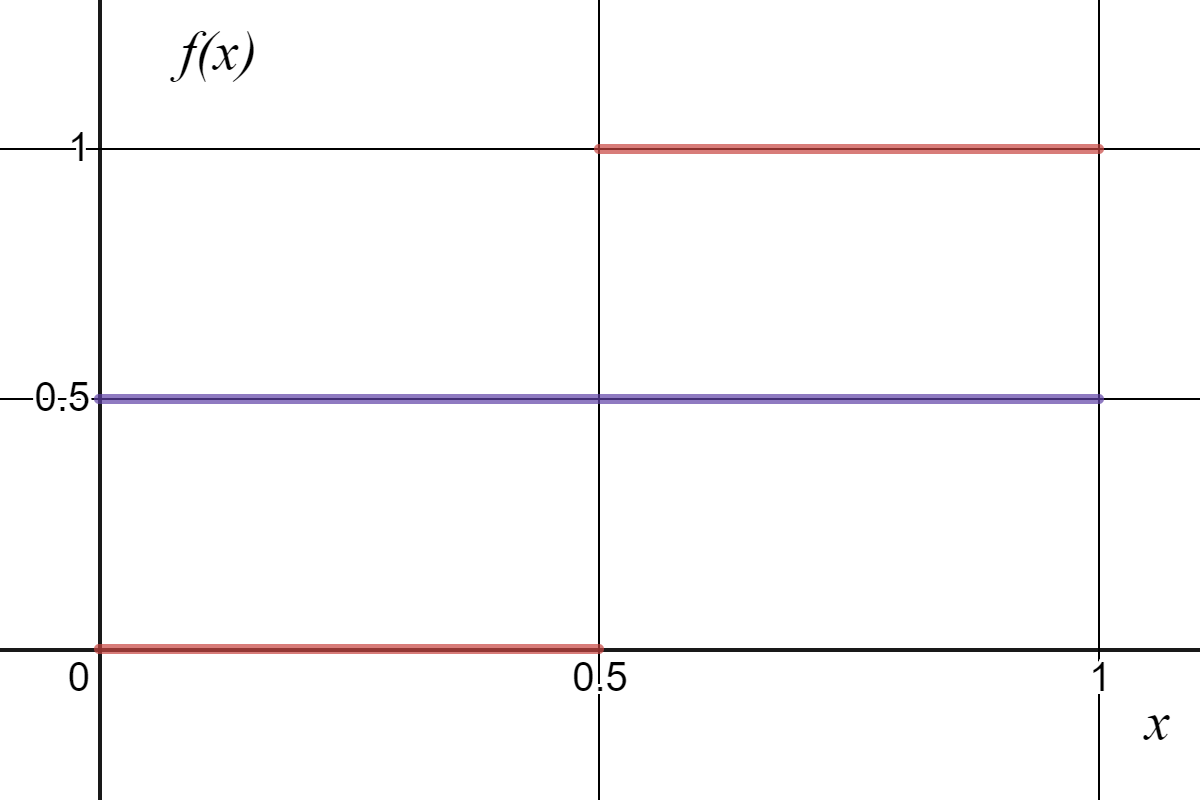
\includegraphics[width=\textwidth]{Figures_Part_5/N=0.png}
				\caption{$N=0$ approximation.}
			\end{subfigure}
			~ 
			\begin{subfigure}[h]{0.3\textwidth}
				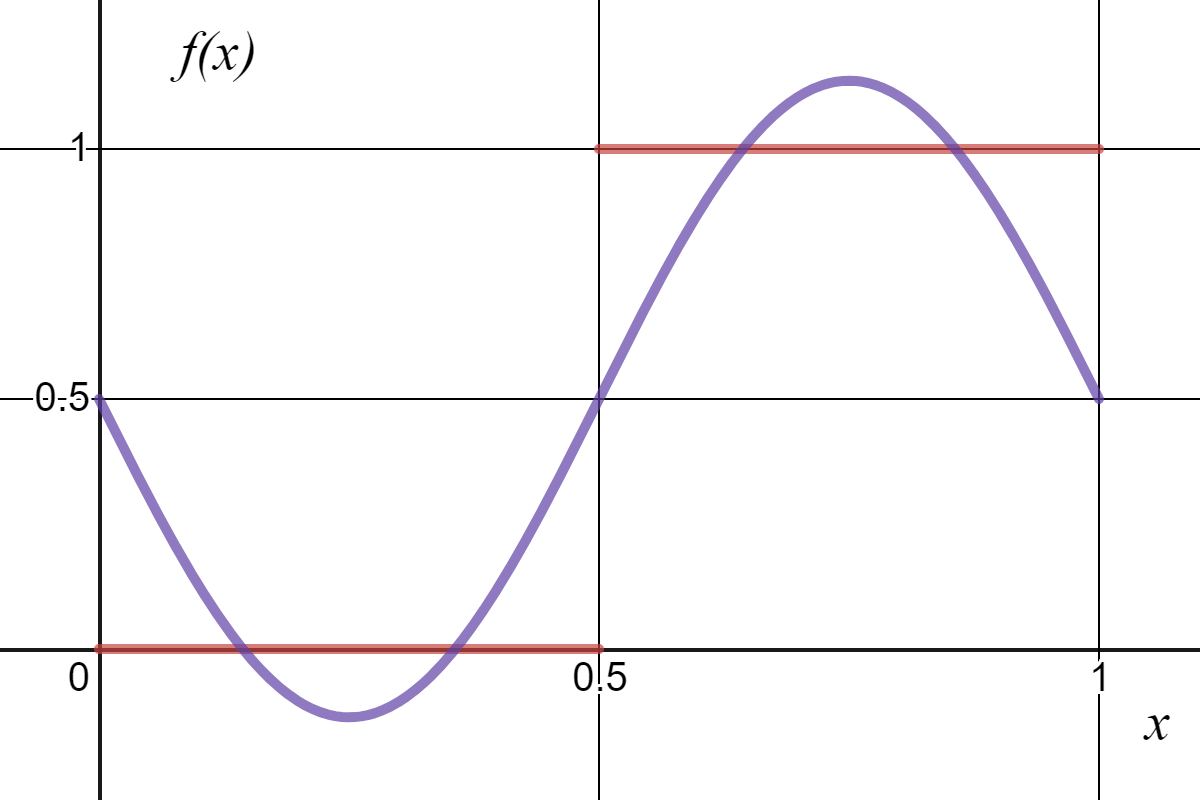
\includegraphics[width=\textwidth]{Figures_Part_5/N=1.png}
				\caption{$N=1$ approximation.}
			\end{subfigure}
			~
			\begin{subfigure}[h]{0.3\textwidth}
				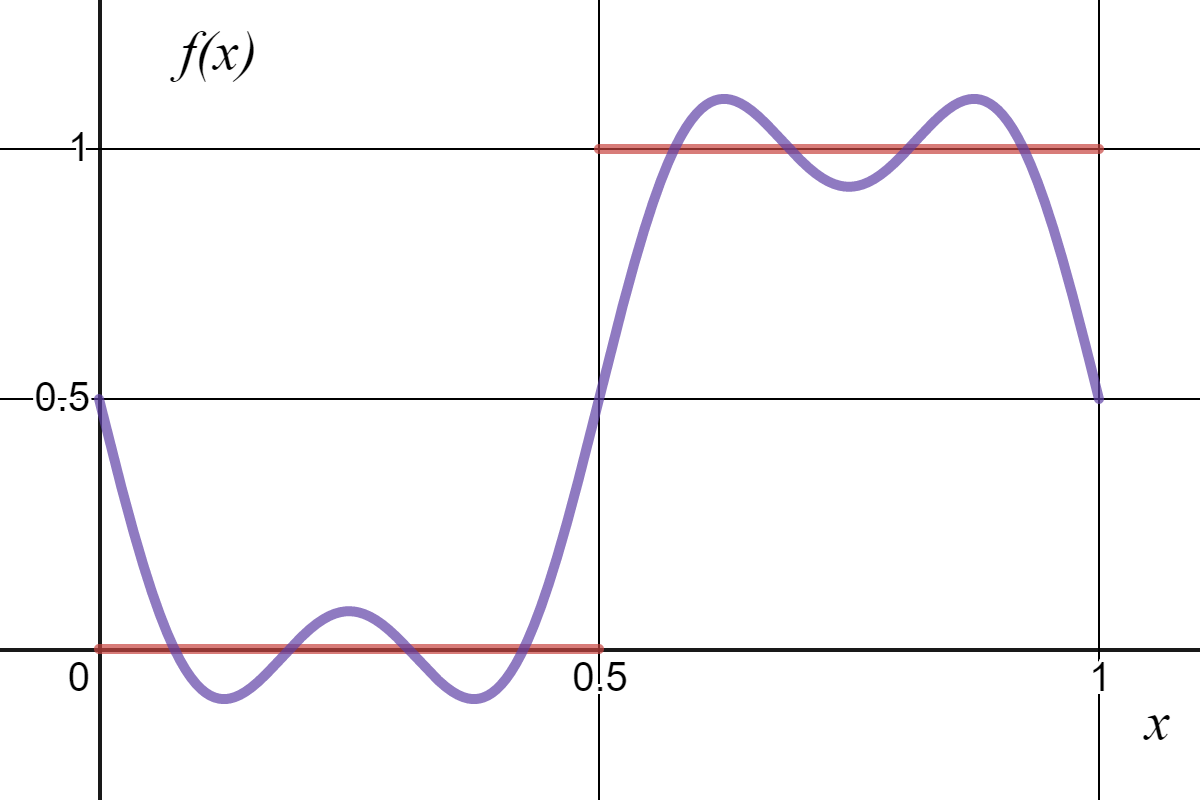
\includegraphics[width=\textwidth]{Figures_Part_5/N=3.png}
				\caption{$N=3$ approximation.}
			\end{subfigure}\\
			
			\begin{subfigure}[h]{0.3\textwidth}
				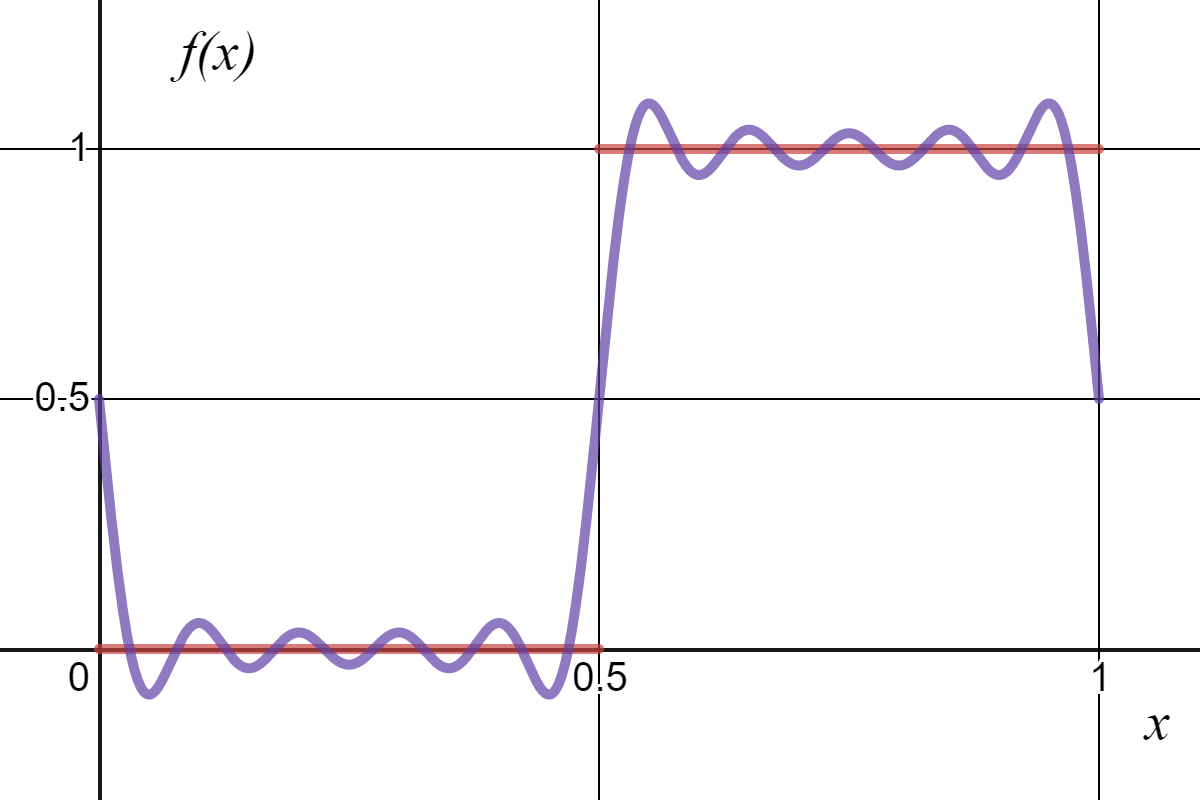
\includegraphics[width=\textwidth]{Figures_Part_5/N=10.png}
				\caption{$N=10$ approximation.}
			\end{subfigure}
			~ 
			\begin{subfigure}[h]{0.3\textwidth}
				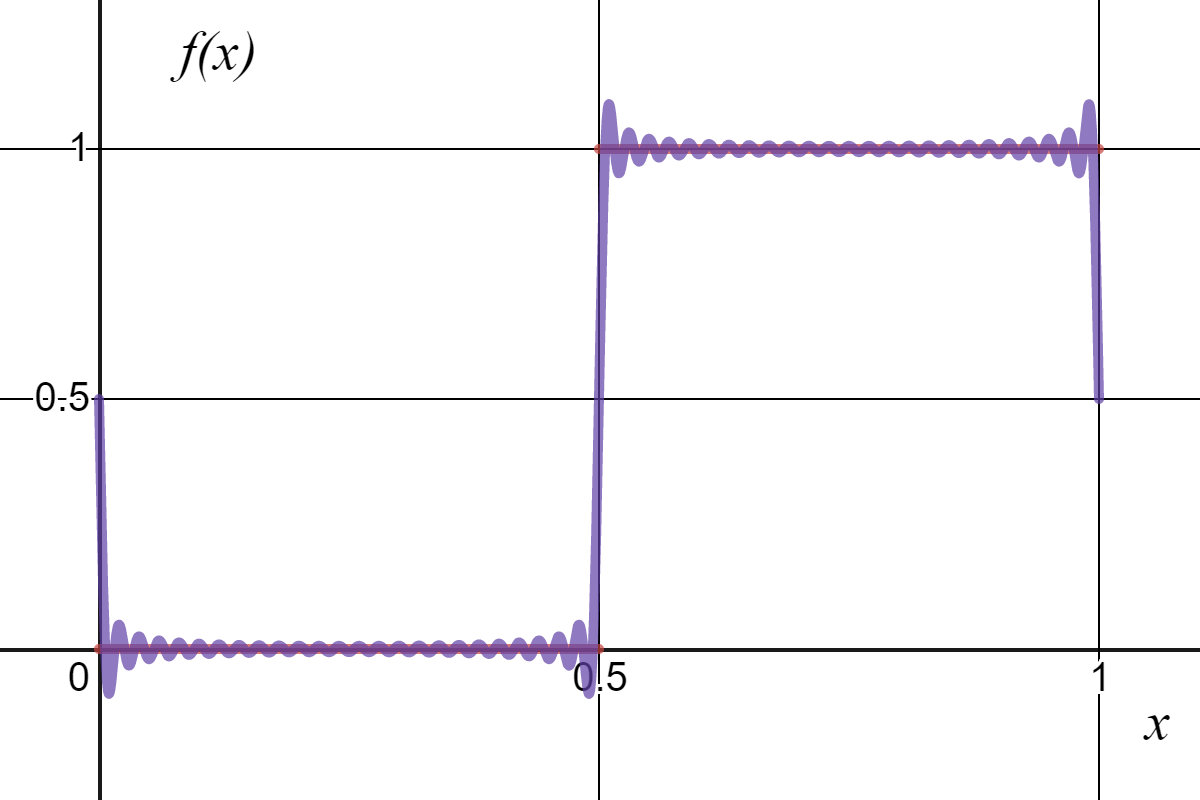
\includegraphics[width=\textwidth]{Figures_Part_5/N=50.png}
				\caption{$N=50$ approximation.}
			\end{subfigure}
			~
			\begin{subfigure}[h]{0.3\textwidth}
				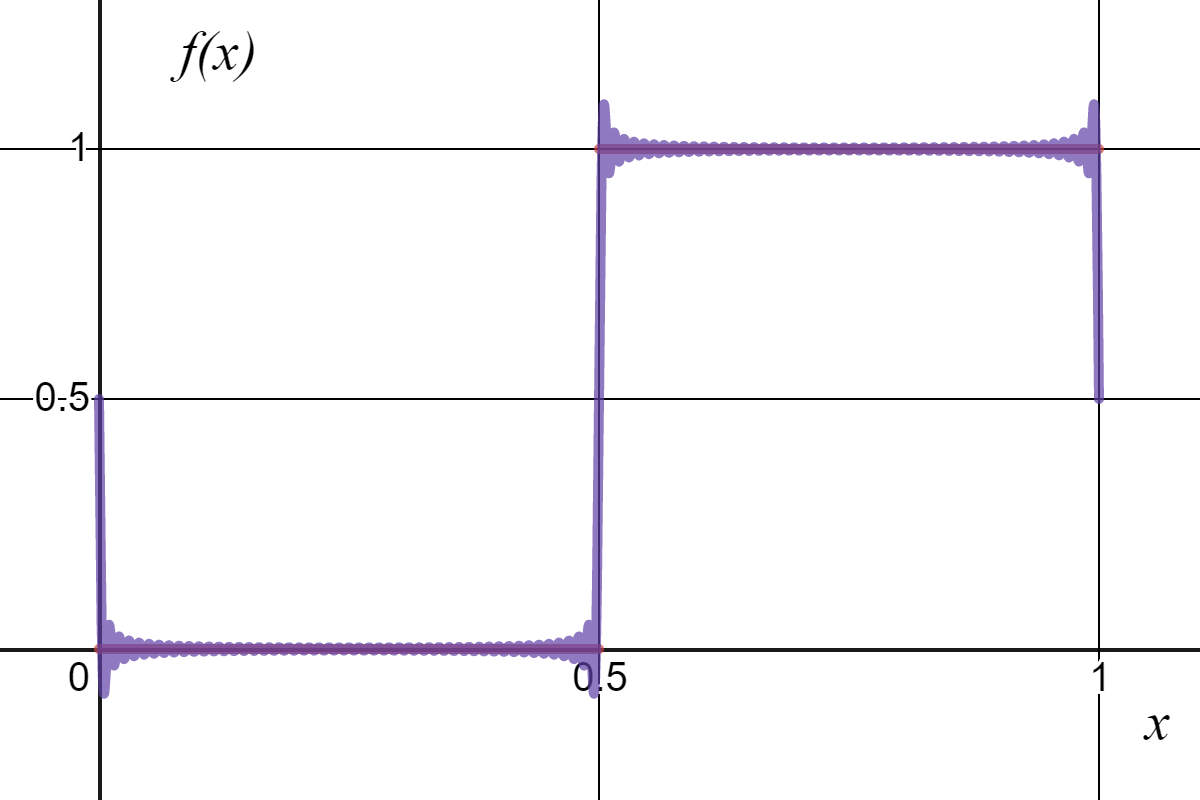
\includegraphics[width=\textwidth]{Figures_Part_5/N=100.png}
				\caption{$N=100$ approximation.}
			\end{subfigure}
		\caption{True $f(x)$ in red. Approximations in purple.}
		\end{figure}
\end{ex}

\section{Fourier Transform}

Let us transition into a more general point of view of the Fourier series.  Specifically, we wish to utilize the Fourier transform.  The idea behind the Fourier transform is to convert a given function $f$ into a new one that we denote by $\hat{f}$ that contains the frequency information of $f$.  This new function will look different, but it will be (in some way) equivalent to our original function. However, we do gain some ability to solve differential equations with the transformed function. 

First, we can rewrite the Fourier series by using complex functions.  Again, we consider functions defined on the interval $[0,L]$ and take the functions
\[
e^{\frac{i 2n \pi x}{L}} \qquad n=\dots, -2,-1,0,1,2,\dots,
\]
as our orthonormal basis functions.  Note that these are indeed normalized when we take the inner product
\begin{align*}
\innprod{e^{\frac{i 2n \pi x}{L}}}{e^{\frac{i 2n \pi x}{L}}} &= \frac{1}{L} \int_0^Le^{\frac{i 2n \pi x}{L}}e^{\frac{-i 2n \pi x}{L}}dx\\
&= \frac{1}{L}\int_0^L 1 dx\\
&= 1.
\end{align*}
In some way we can now see that the functions are a bit more natural to use.  Recall of course that Euler's formula gives us the connection from this representation to the one we previously discussed. That is,
\[
e^{\frac{i 2n \pi x}{L}} = \cos\left(\frac{2n \pi x}{L}\right) + i \sin\left(\frac{2 n \pi x}{L} \right).
\]
Thus, we can write functions by taking the following linear combination
\[
f(x) = \sum_{-\infty}^\infty c_n e^{\frac{i 2n \pi x}{L}},
\]
where the constants $c_n$ are allowed to be complex valued.  Then, the \boldgreen{Fourier transform} of the function $f$, denoted by $\hat{f}$, is given by
\[
\hat{f}(k) = c_k,
\]
is the coefficients of from the Fourier series.  Thus, what we find is that the Fourier transform describes ``how much" of the frequency $\frac{2 k \pi}{L}$ makes up the function $f$.

\begin{ex}{Square Wave Fourier Transform}{square_wave_transform}
	If we consider the square wave function given by
	\[
	f(x) = \begin{cases} 0 & x<L/2 \\ 1 & x\geq L/2, \end{cases},
	\]
	then we can compute the Fourier components with the complex basis functions
	\[
	e^{\frac{ i 2n \pi x}{L}}.
	\]
	Thus, we compute the coefficients in the same by
	\begin{align*}
		c_k &= \innprod{f}{e^{\frac{ i 2n \pi x}{L}}}\\
		&= \frac{ie^{i \pi k}(-1-e^{i\pi k})}{2\pi k}\\
		&= \frac{i(-1)^k (-1-(-1)^k)}{2\pi k}\\
	\end{align*}
	Hence, the Fourier transform of $f$ is given by
	\[
	\hat{f}(k) =  \frac{i(-1)^k (-1-(-1)^k)}{2\pi k}.
	\]
\end{ex}

We'll arrive at the usefulness of the Fourier transform in a bit, but we will first want to consider a yet more general version of the Fourier transform. Instead of taking functions defined solely on the interval $[0,L]$, we can create a transform that works for functions defined on all of $\R$ or any subset.  The difference is this: we now take a basis of functions to be
\[
e^{i2\pi k x} \qquad k \in \R.
\]
That is, instead of taking a discrete set of basis functions, we will now need a continuous set of basis functions.  The reason for this, heuristically, is due to the fact that there can be a full continuum of frequencies for functions defined on $\R$.  The details are suitably more involved than we can get into for a course at this level!

One may now see why we have built up this framework in the way that we did.  It was a bit of a drawn out process, but it allows us to compute the Fourier transform in a consistent way.  Given a function $f(x)$, we can define the Fourier transform by taking the Hermitian inner product for $\R$ and projecting our function onto the basis elements. For example, we have
\[
\hat{f}(k) = \innprod{f}{e^{i2\pi k x}} = \int_{-\infty}^\infty f(x)e^{-i2\pi kx}dx.
\]
And that's really all!  However, one must mention an immensely important function before we compute some examples.

\subsection{Fourier Transform Operator}

Often time, it will be useful to talk of the Fourier transform as an operator. For this, we will use the notation
\[
\fourier{f(x)}= \hat{f}(k).
\]
Later, we will introduce the inverse operation in that 
\[
\fourierinv{\hat{f}(k)}=f(x).
\]
These operators are fundamental in solving differential equations!

One should also note that the Fourier transform is a unitary linear operator.  Specifically, if we have two functions $f$ and $g$ and a constant $\alpha\in \C$, then
\[
\fourier{f(x)+\alpha g(x)} = \hat{f}(k)+\alpha \hat{g}(k).
\]
Now, the operator is unitary since we also have that
\[
\innprod{f}{g} = \innprod{\hat{f}}{\hat{g}},
\]
where the integrals used to evaluate the inner products are taken over the variables $x$ and $k$ respectively.  

The fact that the Fourier transform is a unitary operator is rather important. It means that the transformation does not disturb the measurements one could wish to make. In the same vein, it allows one to work with the transformed function $\hat{f}(k)$ without losing any information about the system. We'll find that working with $\hat{f}(k)$ is often an easier task.

\section{The Dirac Delta Function}

Studying the Fourier theory naturally brings about a very special (generalized) function known as the \boldgreen{Dirac delta function} which we denote by $\delta(x)$.  Quite simply, we define this function via an integral. Specifically, we have for any function $f(x)$ that
\[
\int_{-\infty}^\infty f(x)\delta(x) dx = f(0).
\]
Moreover, if the interval $[a,b]$ contains $0$, we have
\[
\int_a^b f(x)\delta(x) dx = f(0).
\]
We can change the input value for $\delta(x)$ by taking $\delta(x-x_0)$ and we have
\[
\int_{-\infty}^\infty f(x)\delta(x-x_0)dx = f(x_0).
\]
Put in more simple terms, $\delta$ is the function that, when integrated with another function $f$, evaluates that function at a given input value (so long as we integrate over that input value).  

\begin{remark}
	$\delta(x)$ is in fact \underline{not} a function at all. It is something more general known as a distribution. But this fact is not entirely relevant. We will continue to refer to $\delta(x)$ as a function despite this slight misnomer.
\end{remark}

Why should one even consider such a function? For one, it will show up quite readily for us when using the Fourier transform. But, moreover, it is a physically meaningful function in that describes a concentration of mass at a single point.  For example, when studying electromagnetism, one will talk of charged particles. Often, those charged particles are thought of as single points with a charge $q$.  To determine the total charge in a region, one would perform an integral like
\[
\int_{-\infty}^\infty q\delta(x)dx = q
\]
which shows the total charge $q$. The fact that we have $q\delta(x)$ tells us that all of the charge is concentrated at $x=0$.  

One can define the delta function in another convenient manner.  Specifically, via the Fourier transform. One can also show that 
\[
\delta(x) = \int_{-\infty}^\infty 1 e^{-i2\pi kx}dx, 
\]
which means that the $\delta$ function is the Fourier transform of the constant function.  Moreover,
\[
c\delta(x) = \int_{-\infty}^\infty c e^{-i2\pi kx}dx.
\]
One should believe this on an intuitive level since the Fourier transform of a function returns the function's frequency components. A constant function has only a zero frequency component and hence the transform must reflect this.  

\begin{remark}
	Computing these integrals requires tools from complex analysis that we have not seen.  Thus, we will have to blackbox how these integrals are computed in exchange for their usefulness.
\end{remark}

\section{Computing Fourier Transforms}

To see what we are working with, we should compute a few examples. Once again, the techniques to compute these integrals are beyond the scope of this text, but we can show a few results anyways. Our first goal is to see what is meant by frequency components of a function.

If we start with functions with a constant period of oscillation, we can try to digest what the output of the Fourier transform is telling us. We will consider three functions, each with the same period, and compare their transforms.

\begin{ex}{Fourier Transform of Cosine}{fourier_transform_cosine}
	Let us consider the Fourier transform of the function $f(x)=\cos(x)$.  We can compute this transformation by
	\begin{align*}
	\fourier{f(x)} &= \int_{-\infty}^\infty \cos(x)e^{i2\pi kx}dx\\
	&= \frac{\delta\left(k-\frac{1}{2\pi}\right)-\delta\left((k+\frac{1}{2\pi}\right)}{2}.
	\end{align*}
	Here, we can see that the recovered frequency components are where the input to the delta functions are zero. That is,
	\[
	-2\pi k -1 = 0~ \implies ~k= -\frac{1}{2\pi},
	\]
	and
	\[
	1-2\pi k = 0~ \implies ~k=\frac{1}{2\pi}.
	\]
	Recall that the period of $\cos(x)$ is $2\pi$ and hence the frequency $\nu = \frac{1}{2\pi}$. Here, we can see that there is both a $\pm \frac{1}{2 \pi}$.
\end{ex}

In the previous example, one can see how the Fourier transform breaks the function down into frequency components. However, we also know of another function whose frequency is $2\pi$. Namely, $\sin(x)$. Note that these functions are different in that $\cos(x)$ is an even function and $\sin(x)$ is an odd function, so we should expect their Fourier transforms to differ as well (or else this is not an invertible process).

\begin{ex}{Fourier Transform of Sine}{fourier_transform_sine}
	Similarly, we could consider the Fourier transform of the function $f(x)=\sin(x)$.  We'll take
	\begin{align*}
		\fourier{f(x)} &= \int_{-\infty}^\infty \sin(x) e^{i2\pi kx} dx\\
		&= \frac{\delta\left(k-\frac{1}{2\pi}\right)-\delta\left(k+\frac{1}{2\pi}\right)}{2i}
	\end{align*}
	What we see is that the constants in front of the delta functions are different for $\sin(x)$. Specifically, we see the inclusion of the imaginary unit $i$. 
\end{ex}

The differences above display how the Fourier transform is capturing more information about a function than just the frequency information. In some sense, the Fourier transform can determine how even or odd a function is as well.  To finalize this section, let us consider the Fourier transform of another function with frequency $\frac{1}{2\pi}$.

\begin{ex}{Fourier Transform of Complex Exponential}{fourier_transform_exponential}
	Let $f(x)= e^{ix}$, and note that this function has a period of $2\pi$ and hence a frequency of $\frac{1}{2\pi}$.  We can also recall that by Euler's formula, we have
	\[
	e^{ix} = \cos(x)+i\sin(x),
	\]
	and thus we can compute the Fourier transform by
	\begin{align*}
		\fourier{e^{ix}} &= \fourier{\cos(x)+i\sin(x)}\\
		&= \fourier{\cos(x)}+i\fourier{\sin(x)}\\
		&= \delta\left(k-\frac{1}{2\pi}\right)
	\end{align*}
	Again, we find that the Fourier transform captures enough information about our functions to properly differentiate between them.  
\end{ex}

This section would not be complete without some reference of common Fourier transforms.  We'll place a few here, but there are many other references to compute more examples (see for example Wikipedia's page on \emph{Tables of Important Fourier Transforms}.

\begin{table}[H]
        \centering
        \renewcommand{\arraystretch}{2}
        \begin{tabular}{c|c}
            $f(x)$ & $\hat{f}(k)$\\
            \hline
         	$\delta(x)$ & $1$\\
         	$1$ & $\delta(k)$\\
         	$e^{iax}$ & $\delta\left(k-\frac{a}{2\pi}\right)$\\
         	$\cos(ax)$ & $\frac{\delta\left(k-\frac{a}{2\pi}\right)+\delta\left(k+\frac{a}{2\pi}\right)}{2}$\\
     		$\sin(ax)$ & $\frac{\delta\left(k-\frac{a}{2\pi}\right)-\delta\left(k+\frac{a}{2\pi}\right)}{2i}$\\
     		$e^{-\alpha x^2}$ & $\sqrt{\frac{\pi}{\alpha}} e^{\frac{(\pi k)^2}{\alpha}}$
        \end{tabular}
        \label{tab:fourier_transform}
    \end{table}
    
\section{The Inverse Fourier Transform}

The most striking property of the Fourier transform is that it is invertible. Coupled with its linear and unitary nature, the Fourier transform has many nice properties that allow one to make great use of it.  Up until this point, we have only dealt with the forward direction of the Fourier transform. If we are given a function $f(x)$, we can convert this function into $\hat{f}(k)$ which we refer to as the transformed function in the \boldgreen{frequency domain}.  We put
\[
\fourier{f(x)}=\hat{f}(k).
\]
Now, the claim is that this process is invertible in that if we are given a function $\hat{f}(k)$ in the frequency domain, we can convert it back to a function $f(x)$.  That is, we want 
\[
\fourierinv{\hat{f}(k)} = f(x).
\]
Now, since the Fourier transform is a unitary operator, we need only find the adjoint to the Fourier transform.  Recall that, given a unitary operator $\unitop$ we can find $\unitop^{-1}$ by solving
\[
\unitop \unitop^{-1} = I,
\]
where $I$ is the identity. However, the defining property of a unitary operator is that we have
\[
\unitop^{-1} = \unitop^\dagger.
\]
That is, the inverse of a unitary operator is its adjoint! 

Hence, it follows that the \boldgreen{inverse Fourier transform} of a function $\hat{f}(k)$ is given by
\[
f(x) = \int_{-\infty}^\infty \hat{f}(k) e^{i2\pi kx}dk.
\]
If one revisits example \ref{ex:phase_operator}, then we can see that the adjoint to multiplication by a phase is to multiply by the negative phase. That is, the adjoint to $e^{i\theta}$ is $e^{-i\theta}$.  That is the fact that lets us define the inverse Fourier transform above. 

In \ref{tab:fourier_transform}, one can find the inverse Fourier transform of a given function by starting with a $\hat{f}(k)$ and seeing what the corresponding $f(x)$ is.  We'll not worry so much about inverting other functions for now.  

\section{Solving Differential Equations}

Perhaps the most unique feature of the Fourier transform is the transformation of derivatives of a function.  One could in fact argue that this was the true nature of the transformation from the beginning.  Consider a function $f(x)$, then we can differentiate $f(x)$ to get the function $f'(x)$. Now, what is the Fourier transform
\[
\fourier{f'(x)}?
\]
First, (though we have yet to mention this) let us note that any $f(x)$ must be a function that decays rapidly as $x\to \pm \infty$. Let's write this out. We have
\begin{align*}
	\fourier{f'(x)} &= \int_{-\infty}^\infty f'(x)e^{-i2\pi kx}dx\\
	&= i2\pi k \int_{-\infty}^\infty f(x) e^{i2\pi kx}dx\\
	&= i2\pi k \hat{f}(k).
\end{align*}

\begin{exercise}
	Using integration by parts, show that the work above is correct. 
\end{exercise}

What we have found is that the Fourier transform turns derivatives into a multiplication operator! This can be summed up in the following way:
\[
\boxed{\fourier{\frac{d^n}{dx^n} f(x)} = (i2\pi k)^n \hat{f}(k).}
\]

We also have the following as well
\[
\boxed{\fourier{x^n f(x)} = \left(\frac{i}{2\pi}\right)^n \frac{d^n}{dk^n} \hat{f}(k).}
\]
This means that the Fourier transform turns multiplication into differentiation.  

What follows is an algebraic method for solving differential equations. Specifically, any linear differential equation can be quickly transformed into a new (possibly easier) differential equation. The outline can be summarized in the following steps.
\begin{enumerate}[1.]
	\item Take a Fourier transform of both sides of your differential equation.
	\item Solve the new equation for $\hat{f}(k)$ in terms of the frequency variable $k$.
	\item Use the inverse Fourier transform to convert $\hat{f}(k)$ back to $f(x)$.
\end{enumerate}

We'll first start with an example that uses the Fourier series as opposed to the Fourier transform.  Underlying the solution is the same principal, but it gives us a better means for understanding the methodology.

\begin{ex}{Fourier Series Solution of a Second Order Equation}{fourier_series_second_order}
	Consider an elastic band suspended from atop two poles subject to an external force. We can model this equation by
	\[
	-\mu\frac{d^2}{dx^2}f(x) = g(x),
	\]
	with the boundary conditions $f(0)=f(L)=0$. Here, $\mu$ is an elastic constant that describes the stiffness of the elastic.  Then, we let 
	\[
	g(x) = \begin{cases} 0 & x<L/4 \\ 1 & L/4 \leq x < 3L/4 \\ 0 & 3L/4<x \end{cases},
	\]
	which has the following graph.
	\begin{figure}[H]
		\centering
		
\includegraphics[width=.5\textwidth]{Figures_Part_5/square_wave_force.png}
		\caption{A plot of the external force $g(x)$.}
	\end{figure}
	We can also write $g(x)$ as a Fourier series by
	\[
	g(x) = \frac{1}{2}+\sum_{n=1}^{N}\frac{\sin\left(\frac{3\pi n}{2}\right)-\sin\left(\frac{\pi n}{2}\right)}{\pi n}\cos\left(\frac{2n\pi x}{L}\right).
	\]
	Let us also suppose that $f(x)$ is written as a Fourier series,
	\begin{align*}
		f(x) = a_0 + \sum_{n=1}^\infty a_n \sqrt{2} \cos\left(\frac{2n\pi x}{L}\right) + \sum_{n=1}^\infty b_n \sqrt{2} \sin\left(\frac{2n\pi x}{L}\right).
	\end{align*}
	Then, we can plug both Fourier series into the differential equation to get
	\begin{align*}
	\frac{4n^2\pi^2\mu}{L^2} \left(\sum_{n=1}^\infty a_n \sqrt{2} \cos\left(\frac{2n\pi x}{L}\right) + \sum_{n=1}^\infty b_n \sqrt{2} \sin\left(\frac{2n\pi x}{L}\right)\right) \\
	= \frac{1}{2}+\sum_{n=1}^{N}\frac{\sin\left(\frac{3\pi n}{2}\right)-\sin\left(\frac{\pi n}{2}\right)}{\sqrt{2}\pi n}\sqrt{2}\cos\left(\frac{2n\pi x}{L}\right).
	\end{align*}
	Our task now is to solve for the coefficients $a_n$ and $b_n$ and later determine the constant $a_0$ from boundary data. In the above, it's clear that $b_n=0$ and we also have
	\[
	a_n = \frac{L^2\left(\sin\left(\frac{3 n \pi}{2}\right)-\sin\left(\frac{n\pi}{2}\right)\right)}{4\sqrt{2}\pi^3 n^3\mu}.
	\]
	Thus we have the general solution
	\[
	f(x) = a_0 + \frac{1}{\mu}\sum_{n=1}^\infty \frac{L^2\left(\sin\left(\frac{3 n \pi}{2}\right)-\sin\left(\frac{n\pi}{2}\right)\right)}{4\pi^3 n^3} \cos\left(\frac{2n\pi x}{L}\right).
	\]
	Since we require that $f(0)=f(L)=0$ we take
	\[
	0 = f(0)=a_0 + \frac{1}{\mu}\sum_{n=1}^\infty \frac{L^2\left(\sin\left(\frac{3 n \pi}{2}\right)-\sin\left(\frac{n\pi}{2}\right)\right)}{4\pi^3 n^3}.
	\]
	Evaluating the above infinite series gives us
	\[
	0 = a_0 - \frac{1}{64\mu},
	\]
	and so $a_0=\frac{1}{64\mu}$.  Finally, we have our solution
	\[
	\boxed{f(x) = \frac{1}{64\mu}+ \frac{1}{\mu}\sum_{n=1}^\infty \frac{L^2\left(\sin\left(\frac{3 n \pi}{2}\right)-\sin\left(\frac{n\pi}{2}\right)\right)}{4\pi^3 n^3} \cos\left(\frac{2n\pi x}{L}\right).}
	\]
	
	Letting $\mu=\frac{1}{10}$, we can plot our solution.
	\begin{figure}[H]
		\centering
		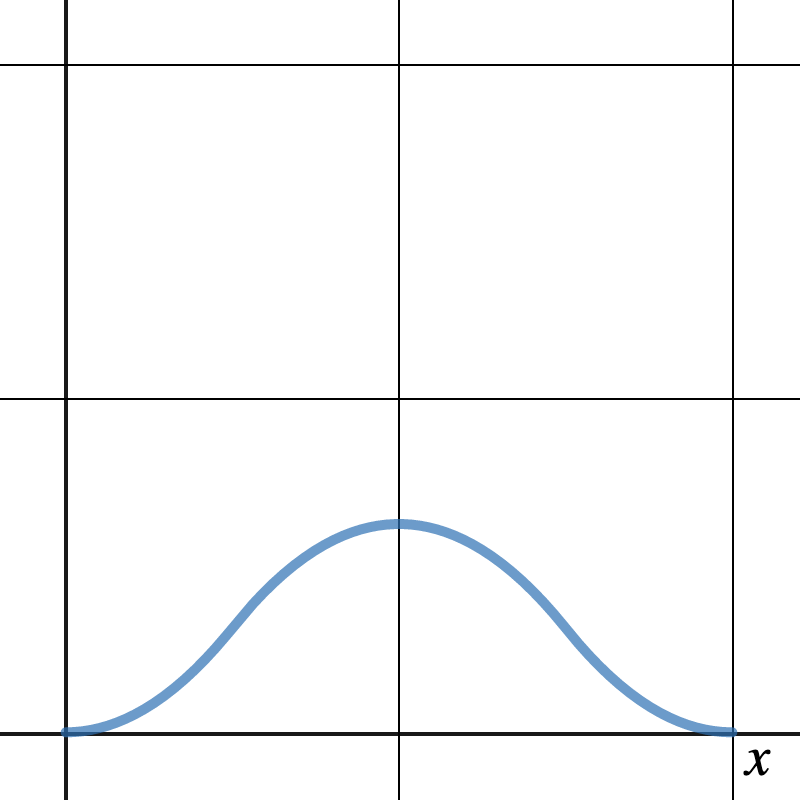
\includegraphics[width=.5\textwidth]{Figures_Part_5/square_wave_diffeq_solution.png}
		\caption{An approximation to the solution $f(x)$ with $N=100$.}
	\end{figure}
\end{ex}
	
\begin{exercise}
	Verify that the Fourier series for $g(x)$ above is correct.
\end{exercise}


\begin{ex}{Fourier Transform Solution of a Second Order Equation}{fourier_transform_second_order}
	Let us consider the same problem as the previous example but with a slightly different approach. We wish to solve the boundary value problem
	\[
	-\mu \frac{d^2}{dx^2} f(x) = g(x)
	\]
	with $f(0)=f(L)=0$ and with 
	\[
	g(x) = \begin{cases} 0 & x<L/4 \\ 1 & L/4 \leq x < 3L/4 \\ 0 & 3L/4<x \end{cases}.
	\]
	Then, we can compute the Fourier transform of $g(x)$ by
	\[
	\hat{g}(k) = \frac{1}{L}\int_0^L g(x)e^{\frac{i2\pi k x}{L}}dx =\frac{e^{ik \pi}\sin\left(\frac{k\pi}{2}\right)}{k \pi}. 
	\]
	Similarly, we can compute the Fourier transform of the left hand side of our differential equation to get
	\[
	\fourier{-\mu \frac{d^2}{dx^2} f(x)} = \mu\frac{4\pi^2k^2}{L^2} \hat{f}(k).
	\]
	Hence, the Fourier transform of the whole differential equation reads
	\[
	\mu\frac{4\pi^2 k^2}{L^2} \hat{f}(k) = \frac{e^{ik \pi}\sin\left(\frac{k\pi}{2}\right)}{k \pi}.
	\]
	Here, we can solve for $\hat{f}(k)$ to get
	\[
	 \hat{f}(k)=\frac{1}{\mu} \frac{L^2 e^{ik \pi}\sin\left(\frac{k\pi}{2}\right)}{4\pi^3k^3}.
	\]
	Inverting the Fourier transform on $[0,L]$ amounts to writing $f(x)$ as the complex Fourier series
	\[
	\boxed{f(x) = \sum_{k=-\infty}^\infty \hat{f}(k) e^{\frac{i2k\pi x}{L}}.}
	\]
\end{ex}

\begin{remark}
	Though arguably less intuitive, the Fourier transform approach is a bit cleaner to work with.  If one were to plot approximations for our function $f(x)$, we would receive the same answer as in the prior example.
\end{remark}

In the previous examples, we were able to solve differential equations on the interval $[0,L]$ whose right hand sides were discontinuous functions.  Prior to this technique, we would have had no way of solving these problems. The further usefulness of the Fourier transform comes into play as we investigate differential equations defined on unbounded sets of $\R$.  For example, we can consider an equation defined on $\R$ with a discontinuous (technically, not even function) right hand side.

\begin{ex}{Fourier Transform for a Second Order Equation on $\R$}{fourier_transform_on_R}
	Consider the following equation
	\[
	-\frac{d^2}{dx^2}f(x) = \delta(x),
	\]
	defined on all of $\R$. We wish to find a general solution for this problem.  To solve this, we take a Fourier transform of both sides of the equation to get
	\[
	4\pi^2 k^2 \hat{f}(k) = 1.
	\]
	We can then solve for the function $\hat{f}(k)$ and get
	\[
	\hat{f}(k) = \frac{1}{4\pi^2 k^2}.
	\]
	Thus, we can then find
	\[
	f(x) = \fourierinv{\frac{1}{4\pi^2k^2}}.
	\]
	Computing this inverse Fourier transform yields
	\[
	\boxed{f(x) = -\frac{|x|}{2}.}
	\]
\end{ex}
	
	
	The above example computes what we refer to as the \boldgreen{fundamental solution} for a differential operator. Specifically, this is when we have a differential operator $\linop$ and we solve
	\[
	\linop f(x) = \delta(x).
	\]
	In our case above, we found the fundamental solution for the 1-dimensional Laplace operator.  If one generalizes this to into 3-dimensions, we will have the equation
	\[
	\nabla \cdot (\nabla V(x,y,z)) = \delta(x,y,z),
	\]
	which garners the solution
	\[
	V(x,y,z) = \frac{1}{4\pi \sqrt{x^2+y^2+z^2}}.
	\]
	This is how one derives the form of the electrostatic potential mathematically!
	
	For now, we will move on to developing calculus in higher dimensions so that we can approach physical problems in space.